%%%%%%%%%%%%%%%%%%%%%%%%%%%%%%%%%%%%%%%%%
% Beamer Presentation
% LaTeX Template
% Version 1.0 (10/11/12)
%
% This template has been downloaded from:
% http://www.LaTeXTemplates.com
%
% License:
% CC BY-NC-SA 3.0 (http://creativecommons.org/licenses/by-nc-sa/3.0/)
%
%%%%%%%%%%%%%%%%%%%%%%%%%%%%%%%%%%%%%%%%%

%----------------------------------------------------------------------------------------
%	PACKAGES AND THEMES
%----------------------------------------------------------------------------------------

\documentclass{beamer}

\mode<presentation> {

% The Beamer class comes with a number of default slide themes
% which change the colors and layouts of slides. Below this is a list
% of all the themes, uncomment each in turn to see what they look like.

%\usetheme{default}
%\usetheme{AnnArbor}
%\usetheme{Antibes}
% \usetheme{Bergen}
%\usetheme{Berkeley}
%\usetheme{Berlin}
%\usetheme{Boadilla}
% \usetheme{CambridgeUS}
%\usetheme{Copenhagen}
%\usetheme{Darmstadt}
%\usetheme{Dresden}
%\usetheme{Frankfurt}
%\usetheme{Goettingen}
%\usetheme{Hannover}
%\usetheme{Ilmenau}
%\usetheme{JuanLesPins}
%\usetheme{Luebeck}
% \usetheme{Madrid}
%\usetheme{Malmoe}
%\usetheme{Marburg}
%\usetheme{Montpellier}
%\usetheme{PaloAlto}
%\usetheme{Pittsburgh}
%\usetheme{Rochester}
%\usetheme{Singapore}
\usetheme{Szeged}
%\usetheme{Warsaw}

% As well as themes, the Beamer class has a number of color themes
% for any slide theme. Uncomment each of these in turn to see how it
% changes the colors of your current slide theme.

% \usecolortheme{albatross}
% \usecolortheme{beaver}
% \usecolortheme{beetle}
% \usecolortheme{crane}
\usecolortheme{dolphin}
% \usecolortheme{dove}
% \usecolortheme{fly}
% \usecolortheme{lily}
% \usecolortheme{orchid}
% \usecolortheme{rose}
% \usecolortheme{seagull}
%\usecolortheme{seahorse}
% \usecolortheme{whale}
%\usecolortheme{wolverine}

%\setbeamertemplate{footline} % To remove the footer line in all slides uncomment this line
%\setbeamertemplate{footline}[page number] % To replace the footer line in all slides with a simple slide count uncomment this line

\setbeamertemplate{navigation symbols}{} % To remove the navigation symbols from the bottom of all slides uncomment this line
}

\setbeamercolor{framesource}{fg=gray}
\setbeamerfont{framesource}{size=\tiny}

\usepackage{graphicx} % Allows including images
\usepackage{booktabs} % Allows the use of \toprule, \midrule and \bottomrule in tables
\usepackage[absolute,overlay]{textpos}
\usepackage{appendixnumberbeamer}
\usepackage{amsmath}

%----------------------------------------------------------------------------------------
% Commands used in this presentation
%----------------------------------------------------------------------------------------

% Lower right image citation
\newcommand{\source}[1]{\begin{textblock*}{4cm}(8.7cm,8.6cm)
    \begin{beamercolorbox}[ht=0.5cm,right]{framesource}
        \usebeamerfont{framesource}\usebeamercolor[fg]{framesource} Source: {#1}
    \end{beamercolorbox}
\end{textblock*}}

% Images in place of math
\newcommand{\mysymbol}[1]{\mathord{\includegraphics[height=1.6cm]{image/#1}}}


%----------------------------------------------------------------------------------------
%	TITLE PAGE
%----------------------------------------------------------------------------------------

\title[Predoctorate Defense]{Bayesian inference methodologies to reconstruct the evolution and spread of pathogens} % The short title appears at the bottom of every slide, the full title is only on the title page

\author{Barney I. Potter} % Your name
\institute[KU Leuven] % Your institution as it will appear on the bottom of every slide, may be shorthand to save space
{
KU Leuven \\ % Your institution for the title page
\medskip
Supervisors: Prof.~Dr.~G. Baele, Dr.~M. Gill
Jury: Prof.~Dr.~G. Opdenakker, Prof.~Dr.~P. Lemey, Prof.~Dr.~J. Matthijnssens, Prof.~Dr.~L. Dupont
}
\date{\today} % Date, can be changed to a custom date

% \logo{
\includegraphics[height=.7cm]{image/KULEUVEN_LOGO_2012.pdf}}

\begin{document}

\begin{frame}
\titlepage % Print the title page as the first slide
\end{frame}

% \begin{frame}
% \frametitle{Overview} % Table of contents slide, comment this block out to remove it
% \colorbox{red}{REMOVE THIS SLIDE FOR FINAL VERSION}
% \tableofcontents % Throughout your presentation, if you choose to use \section{} and \subsection{} commands, these will automatically be printed on this slide as an overview of your presentation
% \end{frame}

%----------------------------------------------------------------------------------------
%	PRESENTATION SLIDES
%----------------------------------------------------------------------------------------

%------------------------------------------------
\section{Introduction} % Sections can be created in order to organize your presentation into discrete blocks, all sections and subsections are automatically printed in the table of contents as an overview of the talk
%------------------------------------------------

\begin{frame}
  \frametitle{Emerging infectious diseases}
  \begin{figure}
    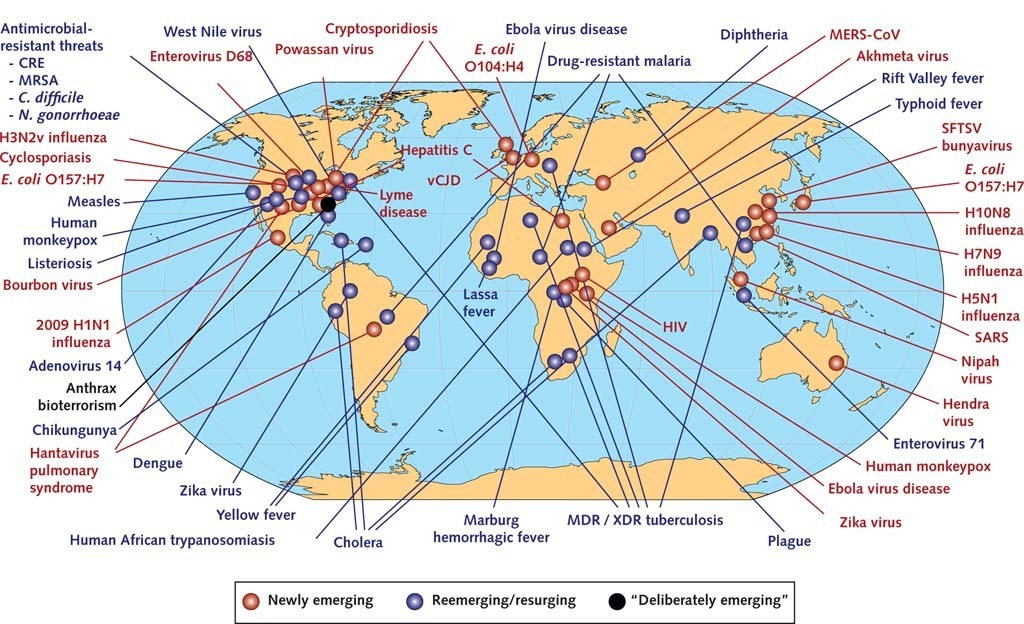
\includegraphics[width=.95\linewidth]{image/intro/eids}
    \source{Paules, 2017}
  \end{figure}
\end{frame}

%------------------------------------------------

\begin{frame}
  \frametitle{Epidemic process}
\end{frame}

%------------------------------------------------

\begin{frame}
  \frametitle{Tree space is enormous}
  \begin{columns}[c]

    \column{.45\textwidth}
      Tree space size:

      $$
      \frac{(2n-3)!}{2^{n-1}(n-1)!}
      $$

    \column{.5\textwidth}
    \begin{table}
      \begin{tabular}{l l}
      \toprule
      \textbf{Species} & \textbf{\# of trees}\\
      \midrule
      1 & 1\\
      2 & 1\\
      3 & 3\\
      4 & 15\\
      5 & 105\\
      6 & 945\\
      7 & 10,395\\
      8 & 135,135\\
      9 & 2,027,025\\
      $\vdots$ & $\vdots$\\
      746 & $2.829\times10^{2037}$\\
      \bottomrule
      \end{tabular}
    \end{table}
  \end{columns}
\end{frame}

%------------------------------------------------

\begin{frame}
  \frametitle{Bayesian phylogenetic inference}
  \begin{columns}[c]

    \column{0.45\textwidth}
      $$
      P(\Theta \vert Data) = \frac{P(Data \vert \Theta)P(\Theta)}{P(Data)}
      $$

      % \begin{alignat*}{}
      %   \Theta \subseteq &\mysymbol{sedes}&, &\mysymbol{sedes},\\
      %                    &\mysymbol{sedes}&, &\mysymbol{sedes}
      % \end{alignat*}

    \column{.5\textwidth}
      Image goes here

  \end{columns}
\end{frame}

%------------------------------------------------
\section{HBV phylogeography}
%------------------------------------------------

\begin{frame}
  \frametitle{What is HBV?}
  \begin{columns}[c] % The "c" option specifies centered vertical alignment while the "t" option is used for top vertical alignment

    \column{.45\textwidth} % Left column and width
      \begin{itemize}
        \item Affects $> 350$ million people annually
        \item Partially dsDNA virus
        \begin{itemize}
          \item Long strand: ~3 kb
          \item Short strand: ~2.2 kb
        \end{itemize}
      \end{itemize}

    \column{.5\textwidth} % Right column and width
      \begin{figure}
        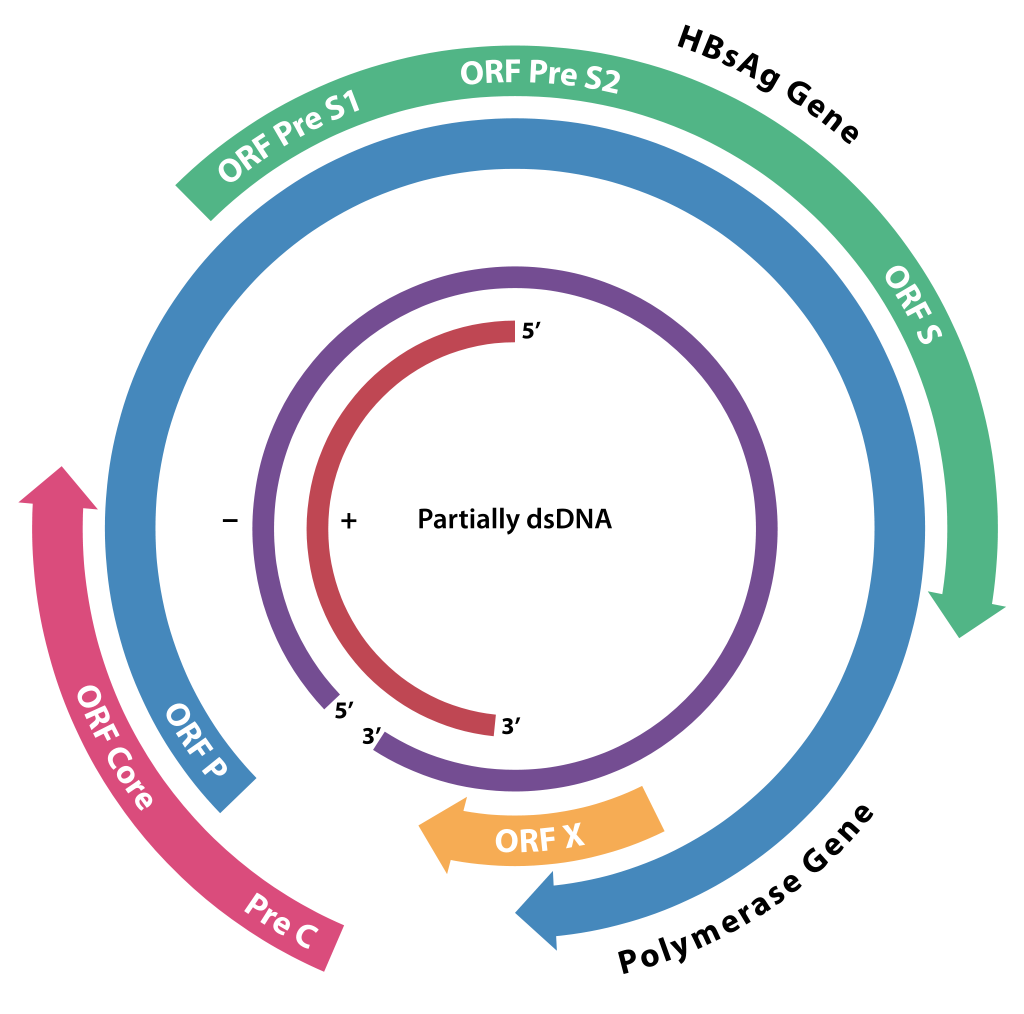
\includegraphics[width=.95\linewidth]{image/results/hbv_genome_schematic}
        \source{Wikimedia commons}
      \end{figure}

  \end{columns}
\end{frame}

%------------------------------------------------
\subsection{Subgenotyping}

\begin{frame}
  \frametitle{Criteria for subgenotyping}
  \begin{itemize}
    \item Phylogenetic placement
    \item Between $4\%-8\%$ nucleotide divergence
    \item
  \end{itemize}
\end{frame}

%------------------------------------------------

\begin{frame}
  \frametitle{HBV-A subgenotyping}
  \begin{figure}
    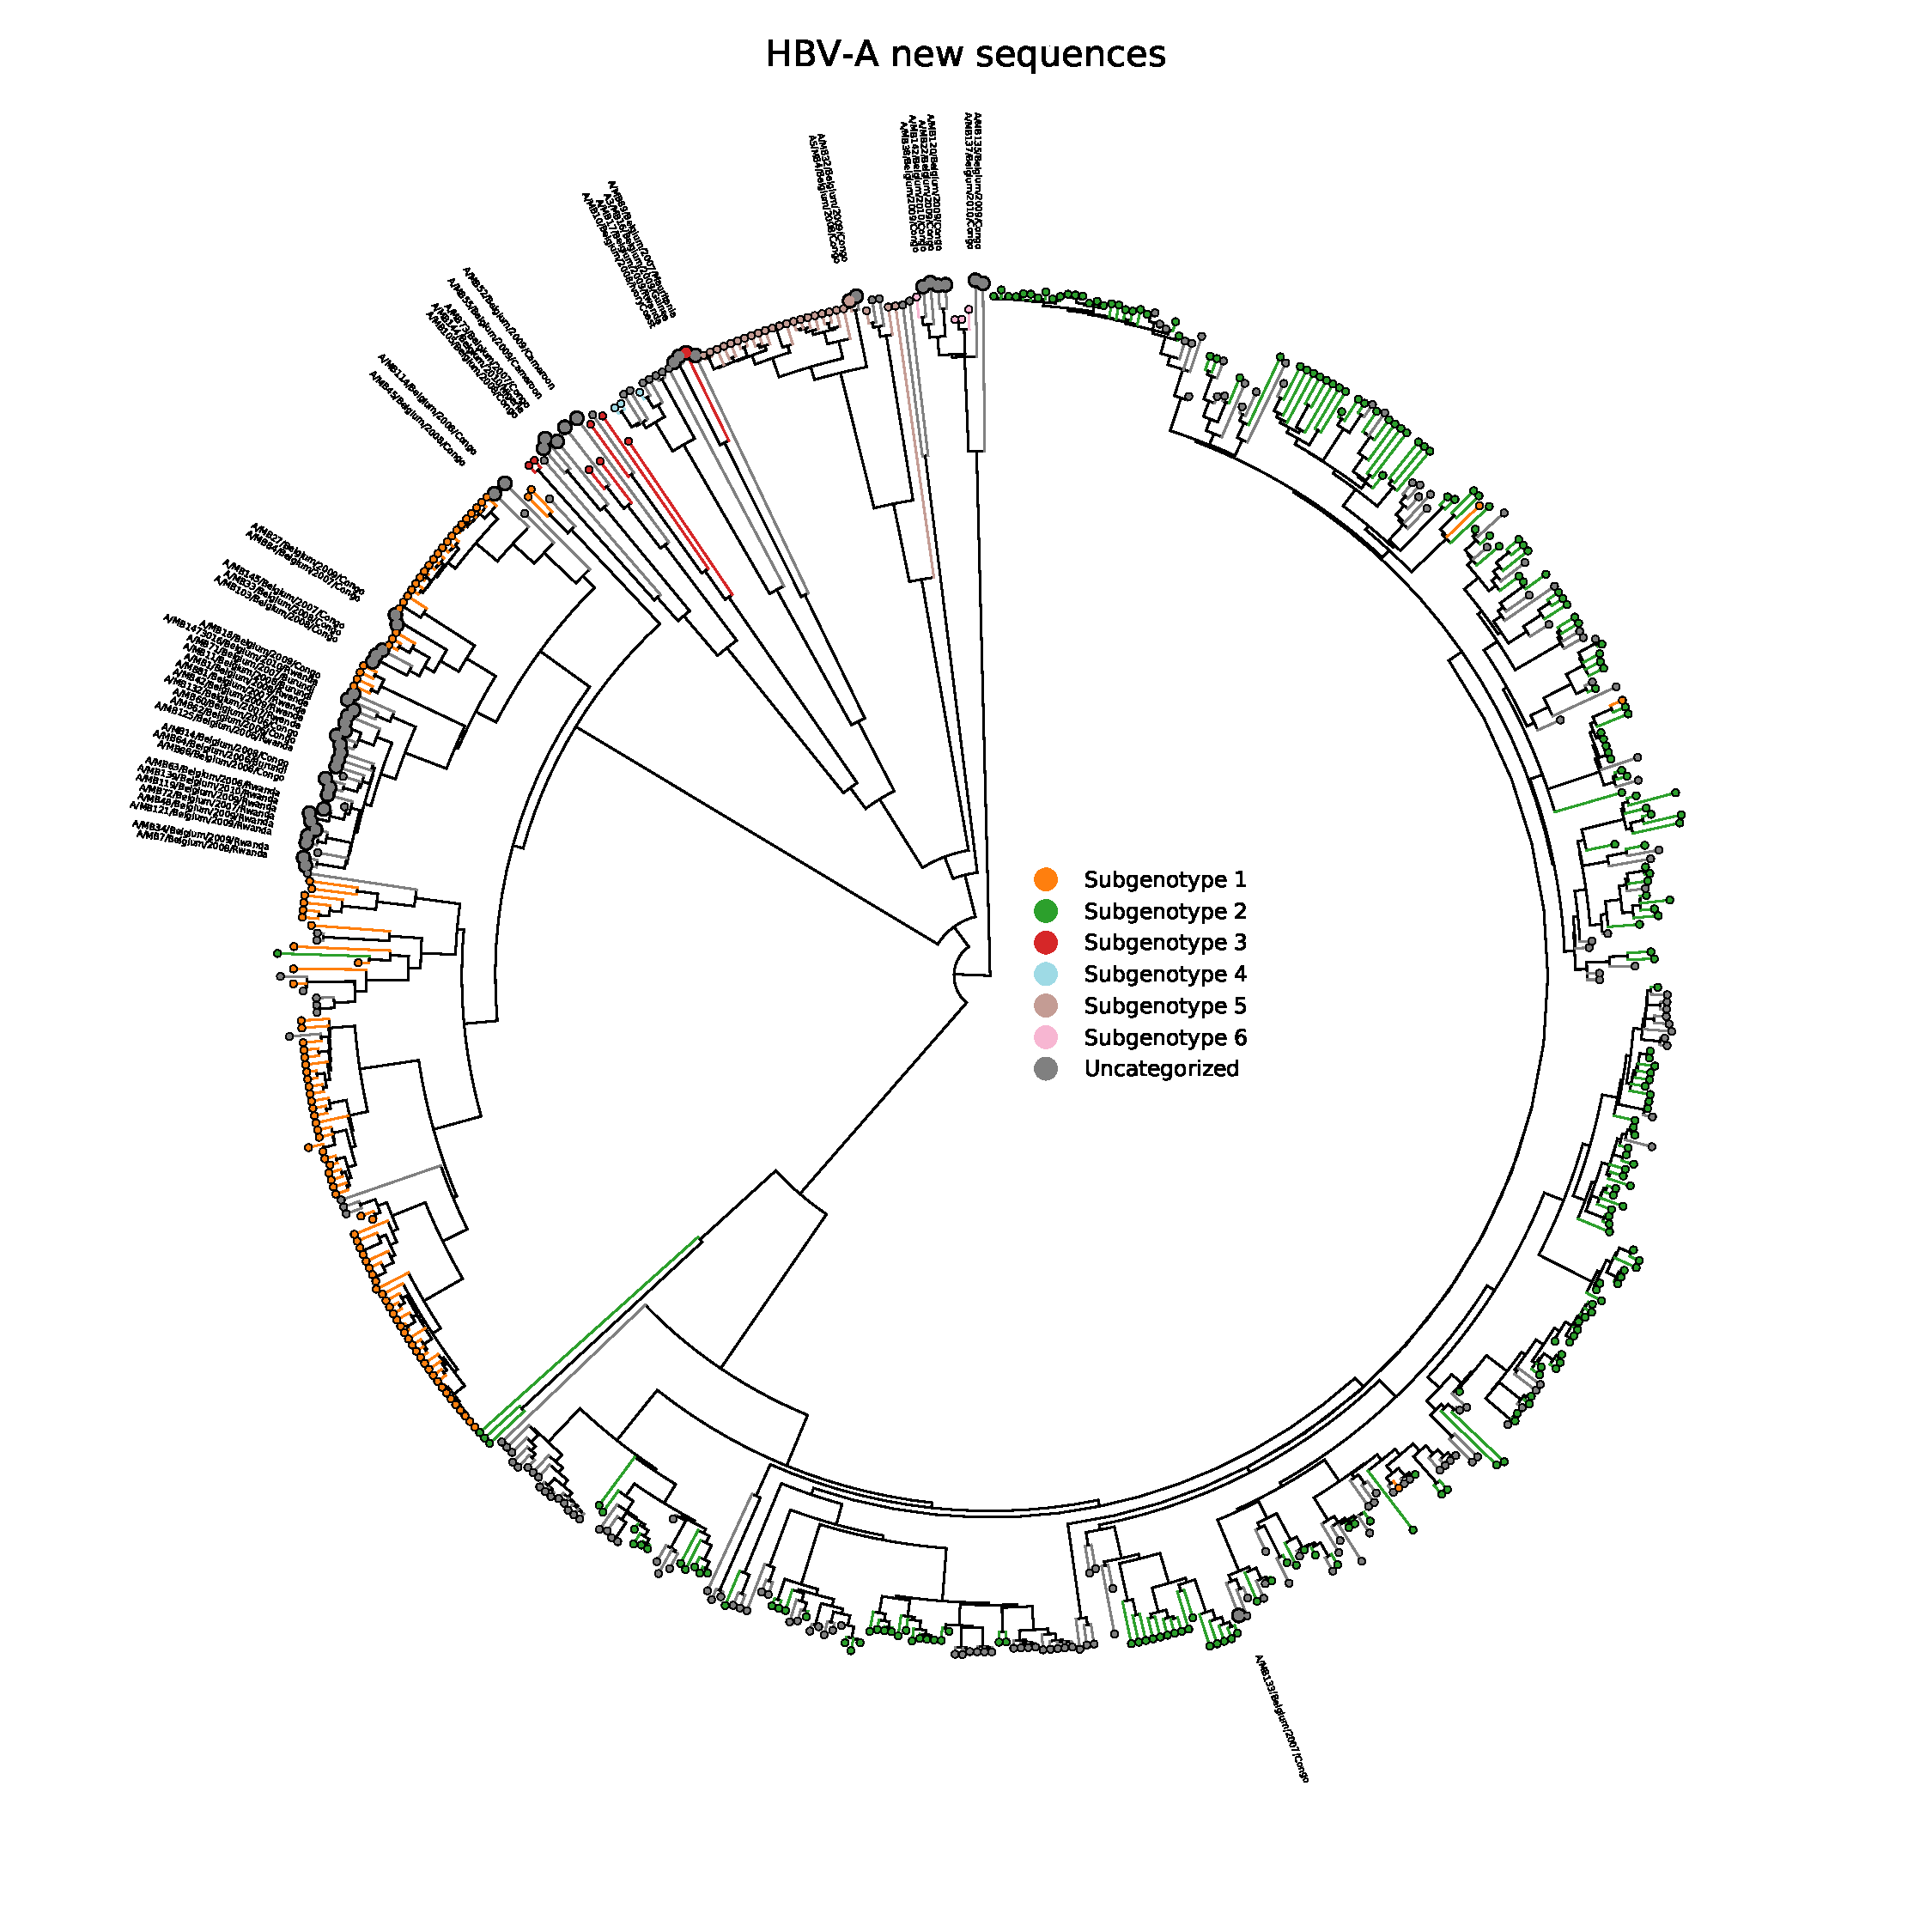
\includegraphics[width=.6\linewidth]{image/results/HBV-A_new_sequences}
  \end{figure}
\end{frame}

%------------------------------------------------

\begin{frame}
  \frametitle{HBV-A subgenotyping}
  \begin{figure}
    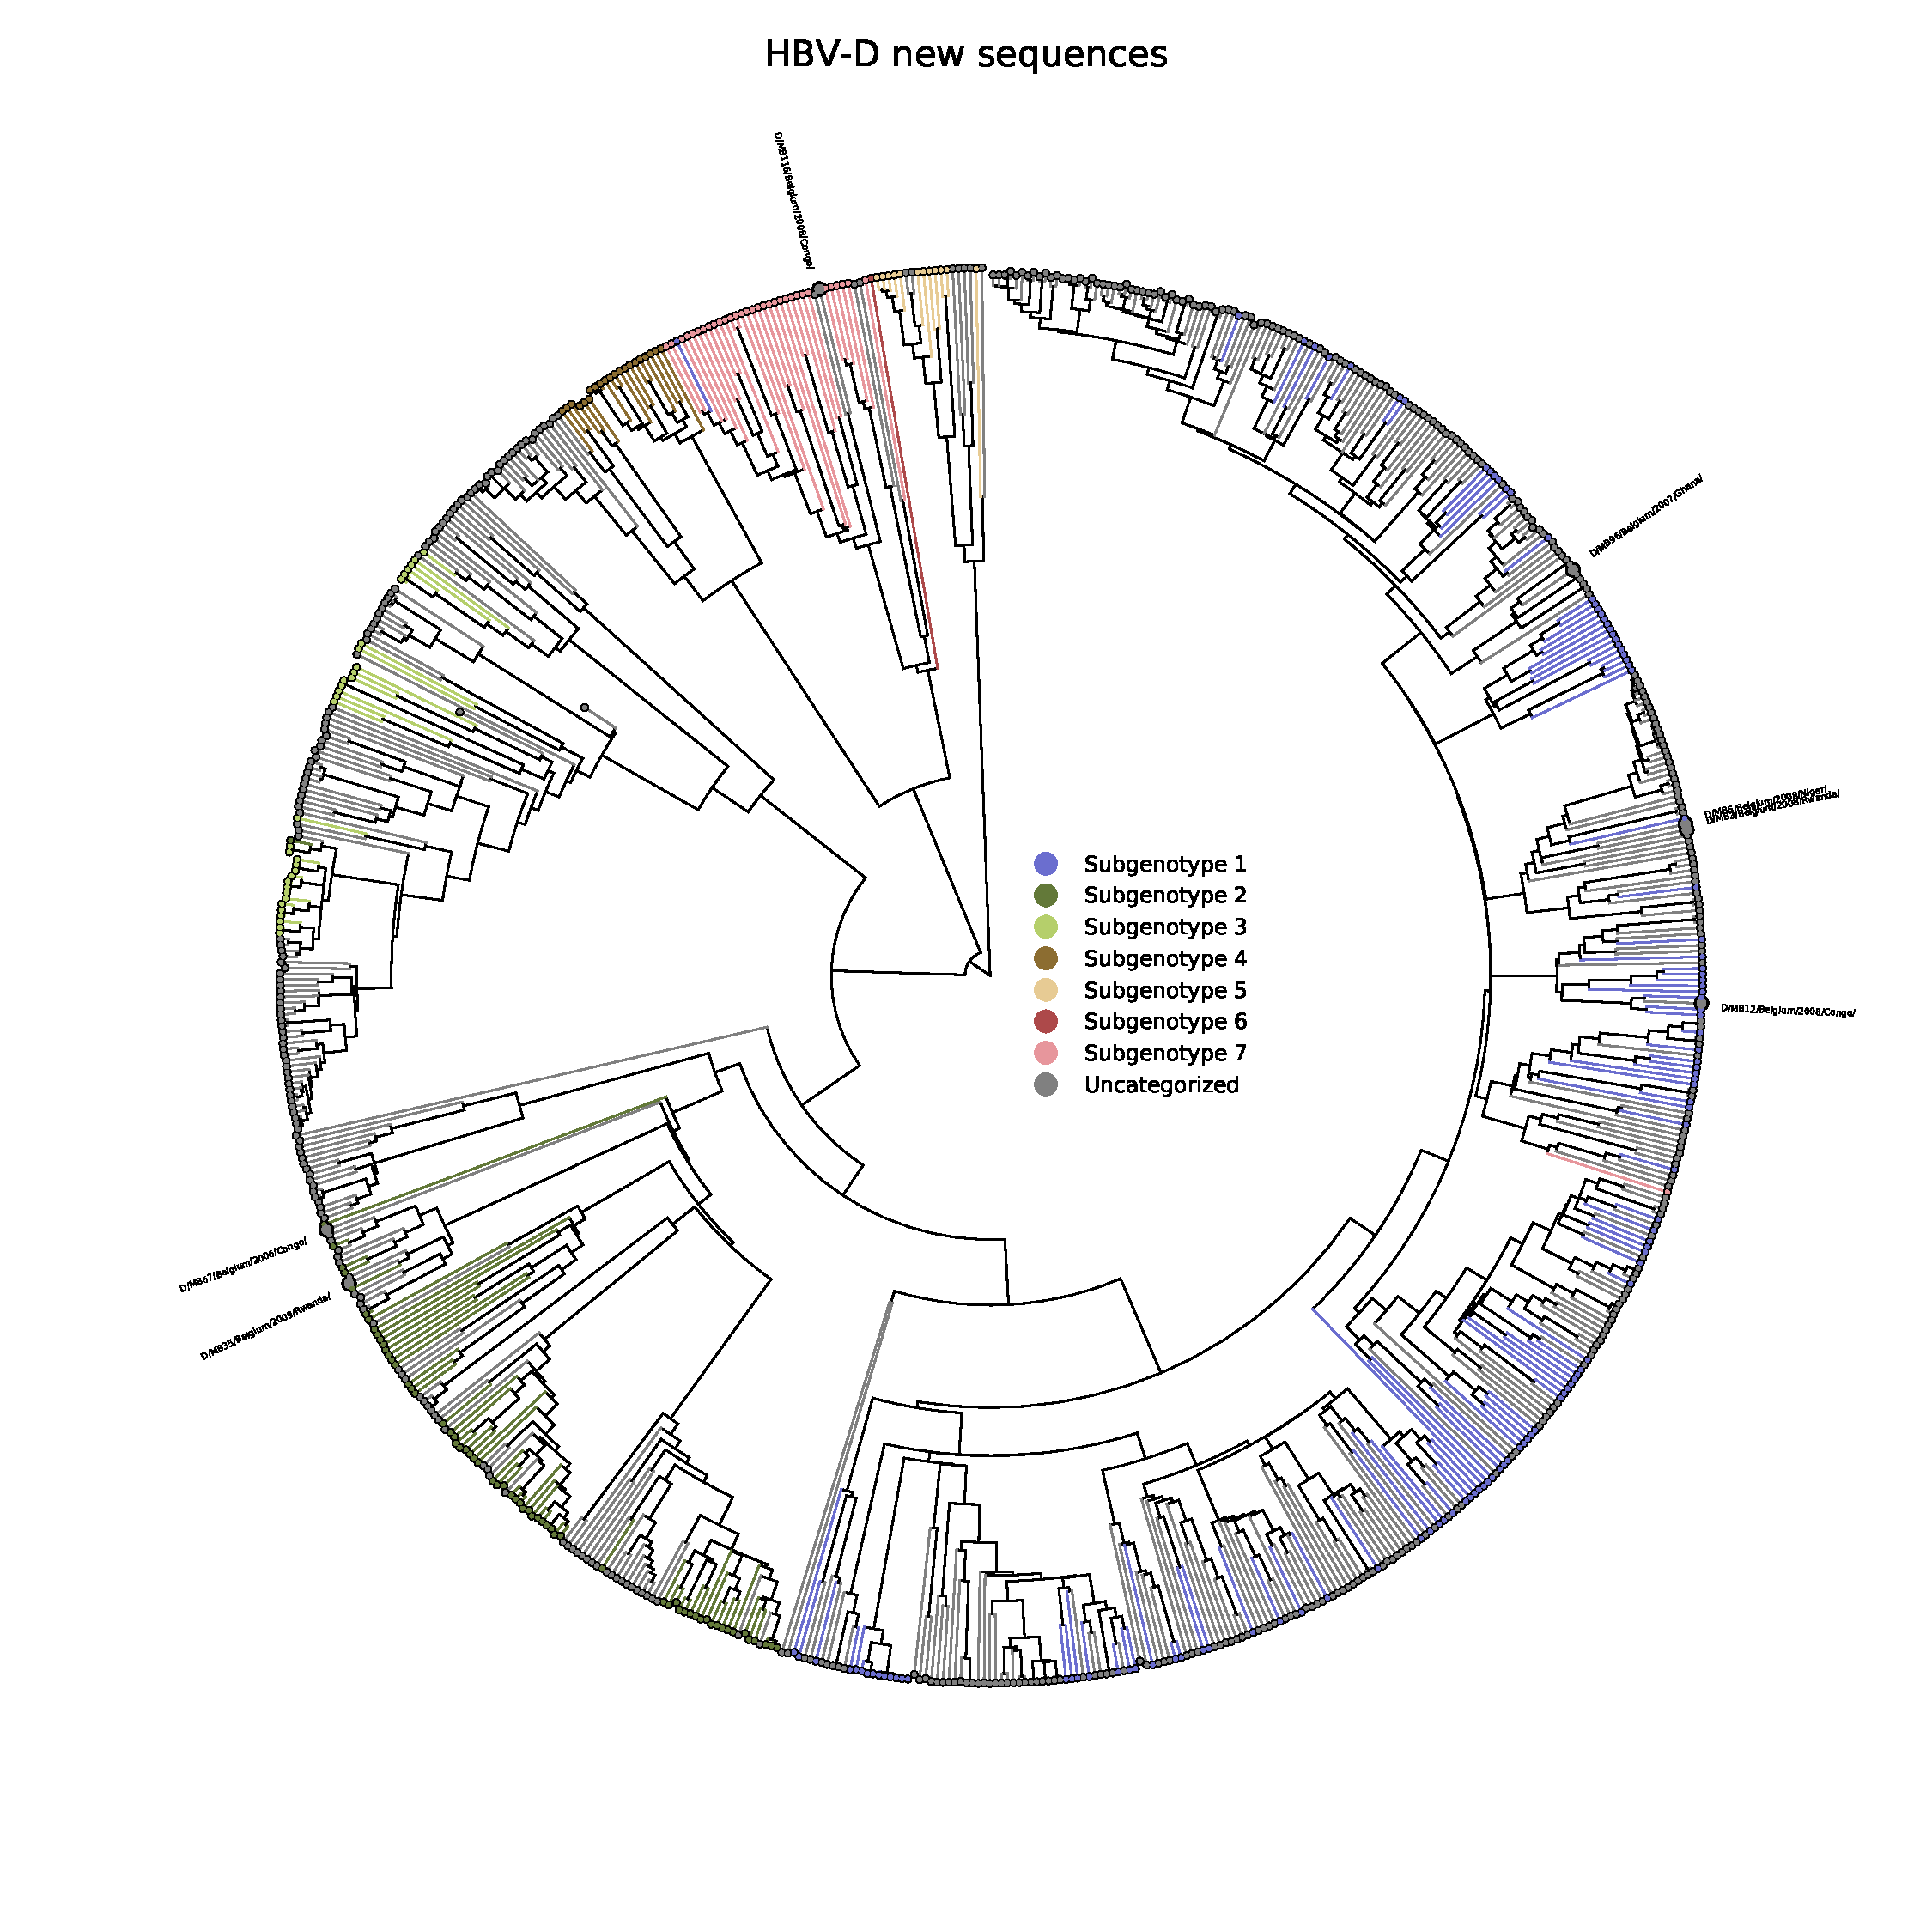
\includegraphics[width=.6\linewidth]{image/results/HBV-D_new_sequences}
  \end{figure}
\end{frame}

%------------------------------------------------
\subsection{Phylogeography}

\begin{frame}
  \frametitle{Objectives}
  Reconstruct evolutionary and migration history of three HBV genotypes (A, D, E):
  \begin{itemize}
    \item Where did each genotype originate?
    \item When were the major migrations of each genotype?
    \item How many times did each genotype move between regions?
  \end{itemize}
\end{frame}

%------------------------------------------------

\begin{frame}
  \frametitle{Methodology}
\end{frame}

%------------------------------------------------

\begin{frame}
  \frametitle{HBV-A}
  \begin{figure}
    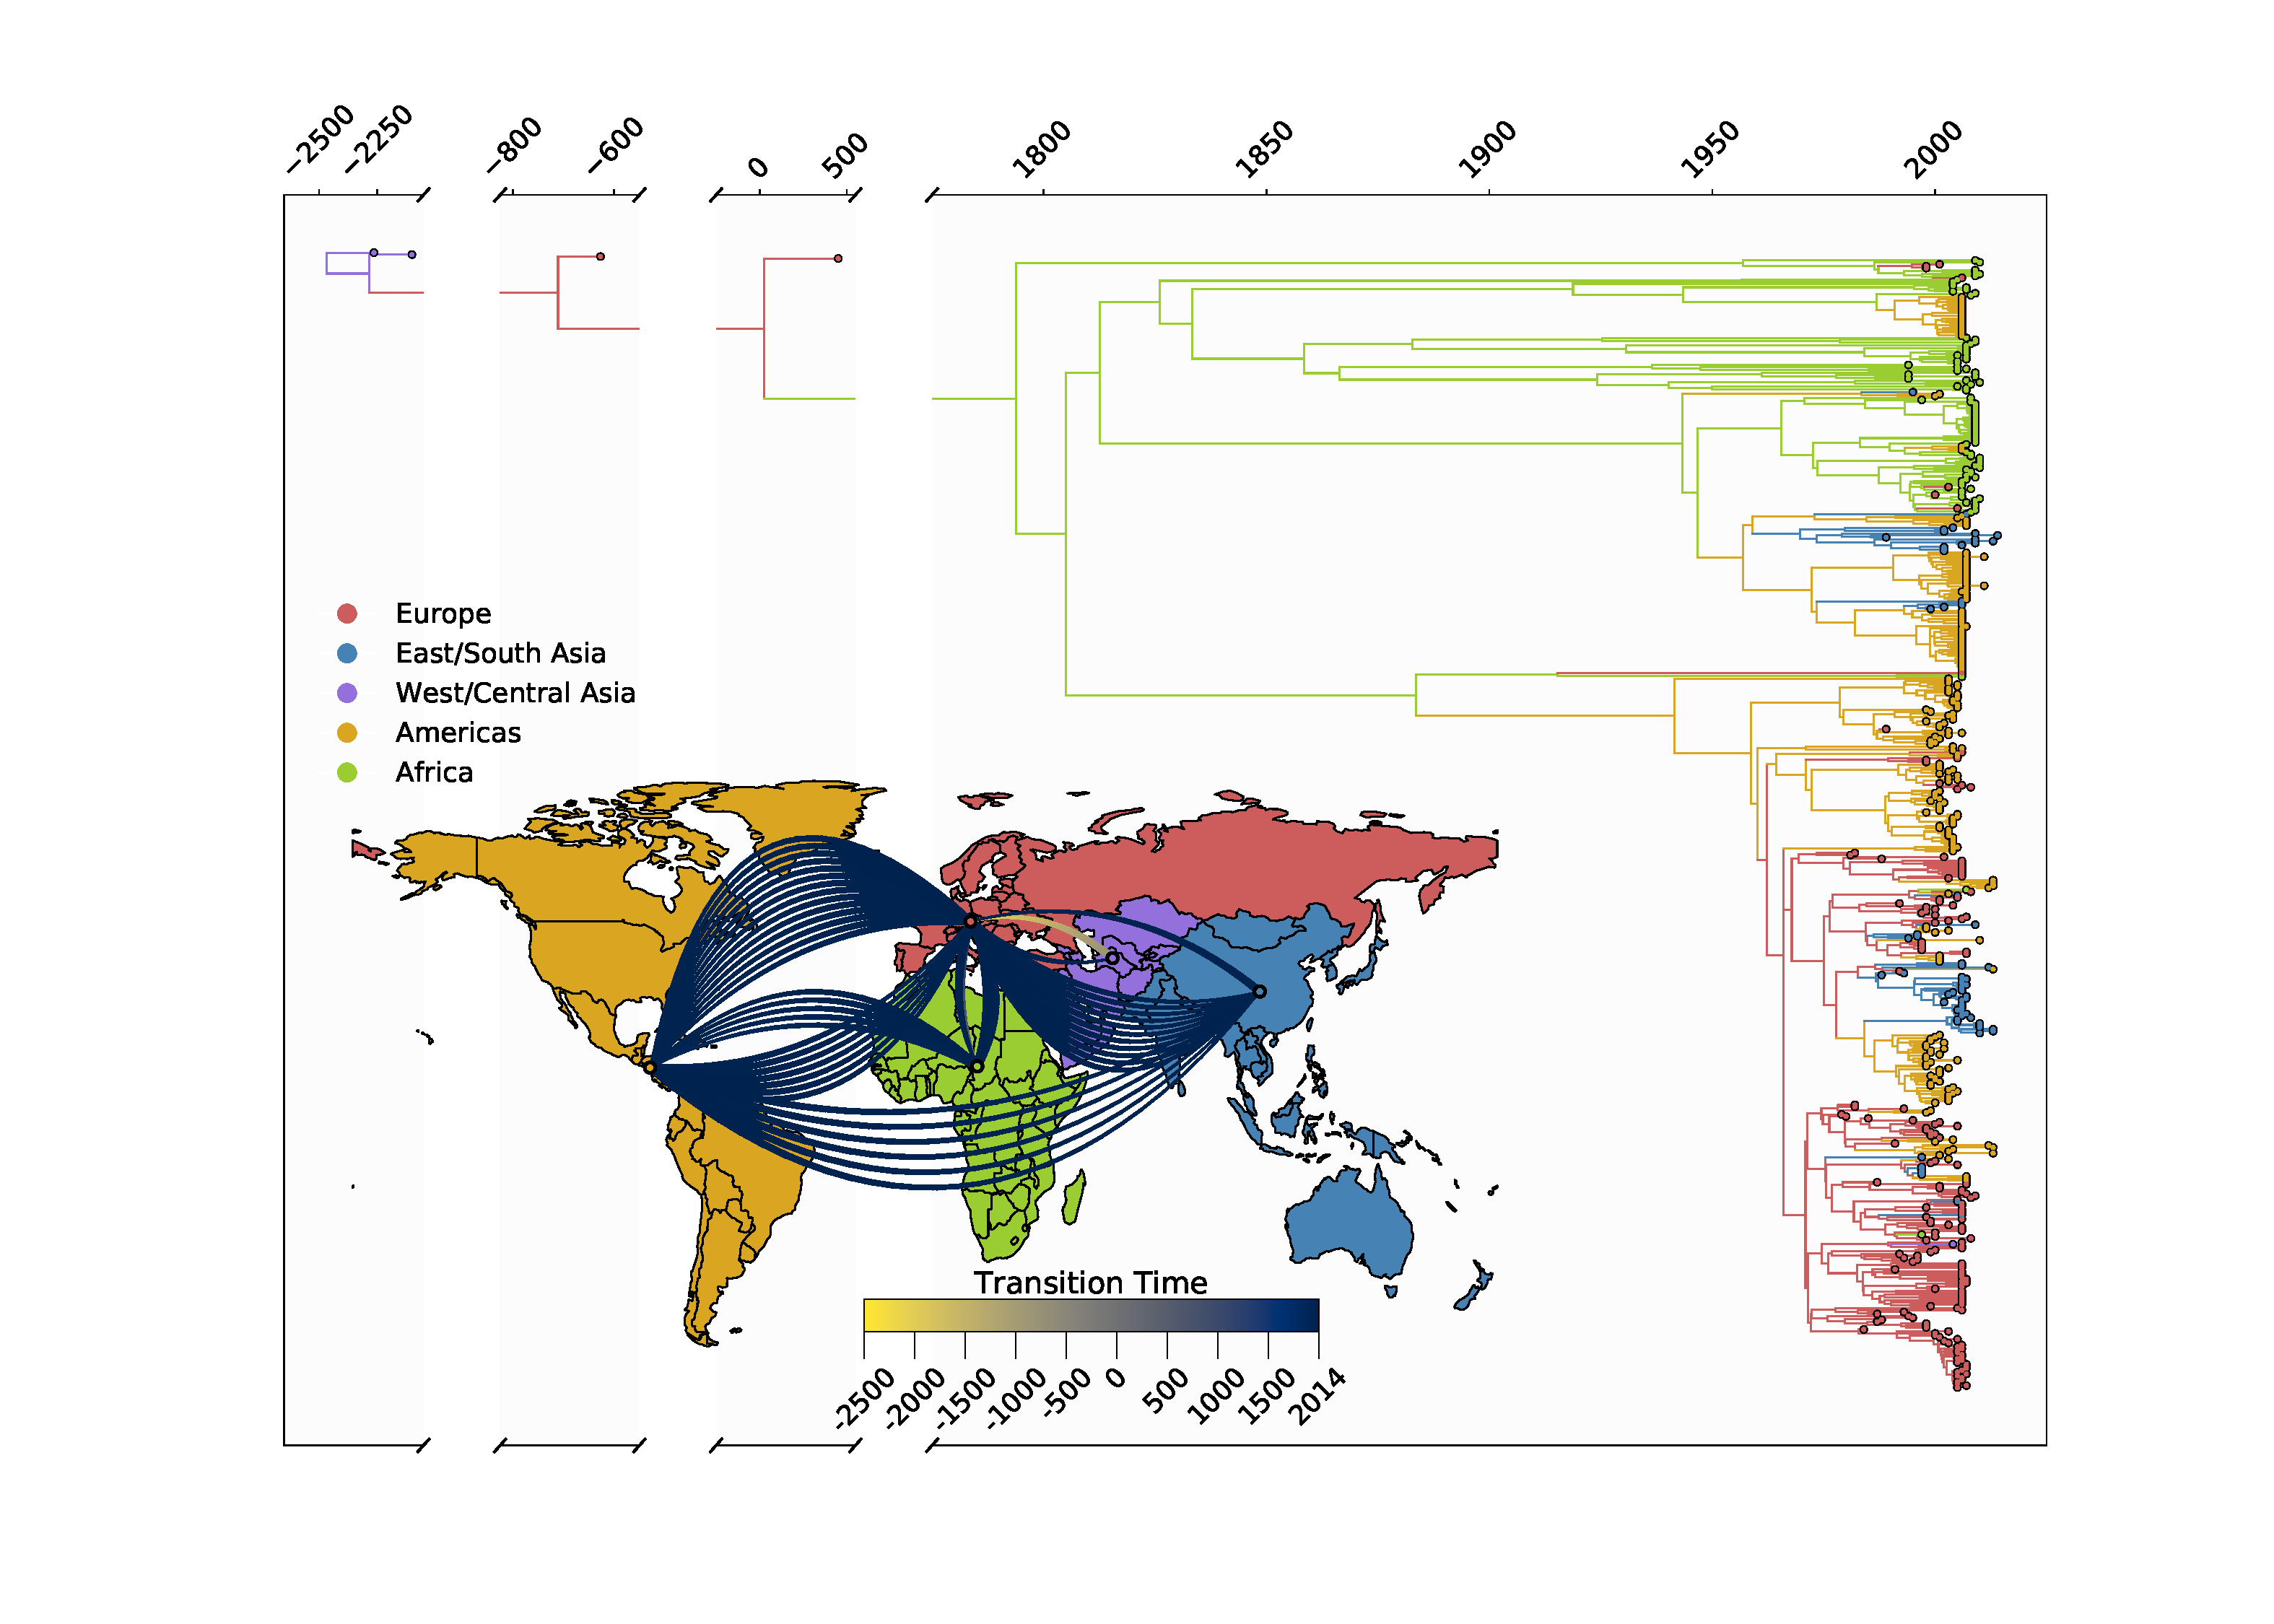
\includegraphics[width=.6\linewidth]{image/results/HBV-A_phylogeography_and_mcc_tree}
  \end{figure}
\end{frame}

%------------------------------------------------

\begin{frame}
  \frametitle{HBV-D}
  \begin{figure}
    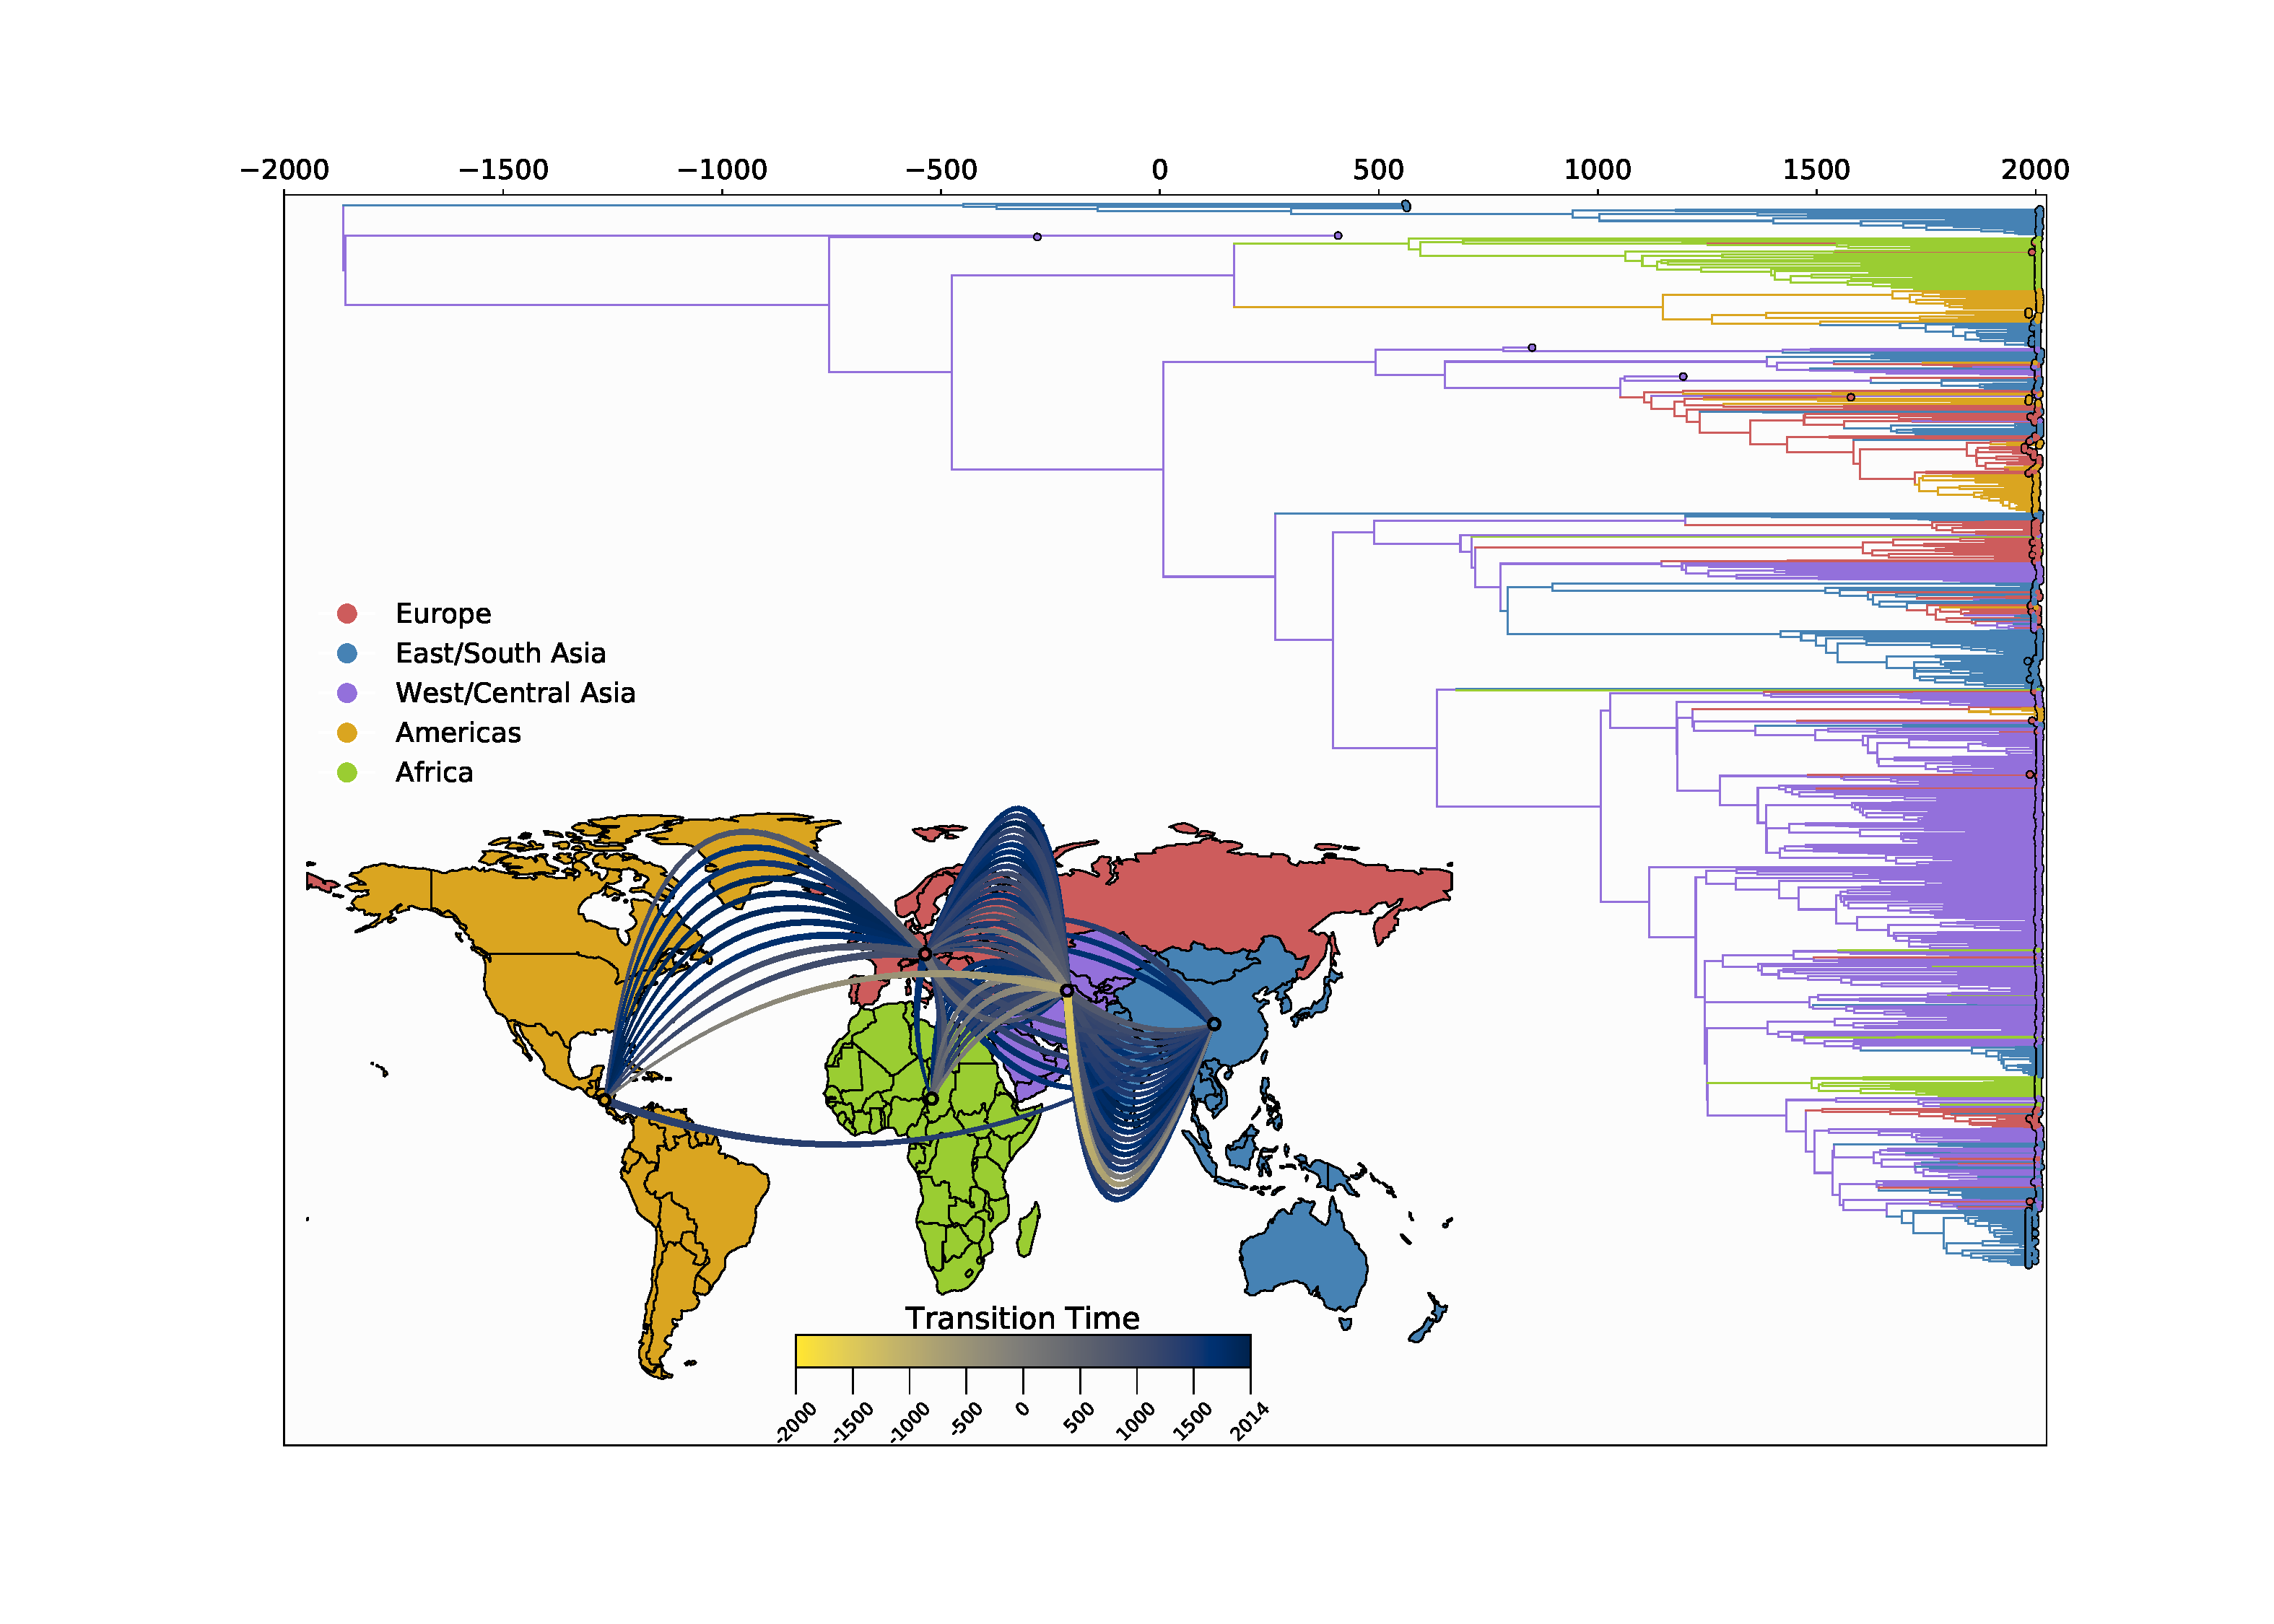
\includegraphics[width=.6\linewidth]{image/results/HBV-D_phylogeography_and_mcc_tree}
  \end{figure}
\end{frame}

%------------------------------------------------

\begin{frame}
  \frametitle{HBV-E}
  \begin{figure}
    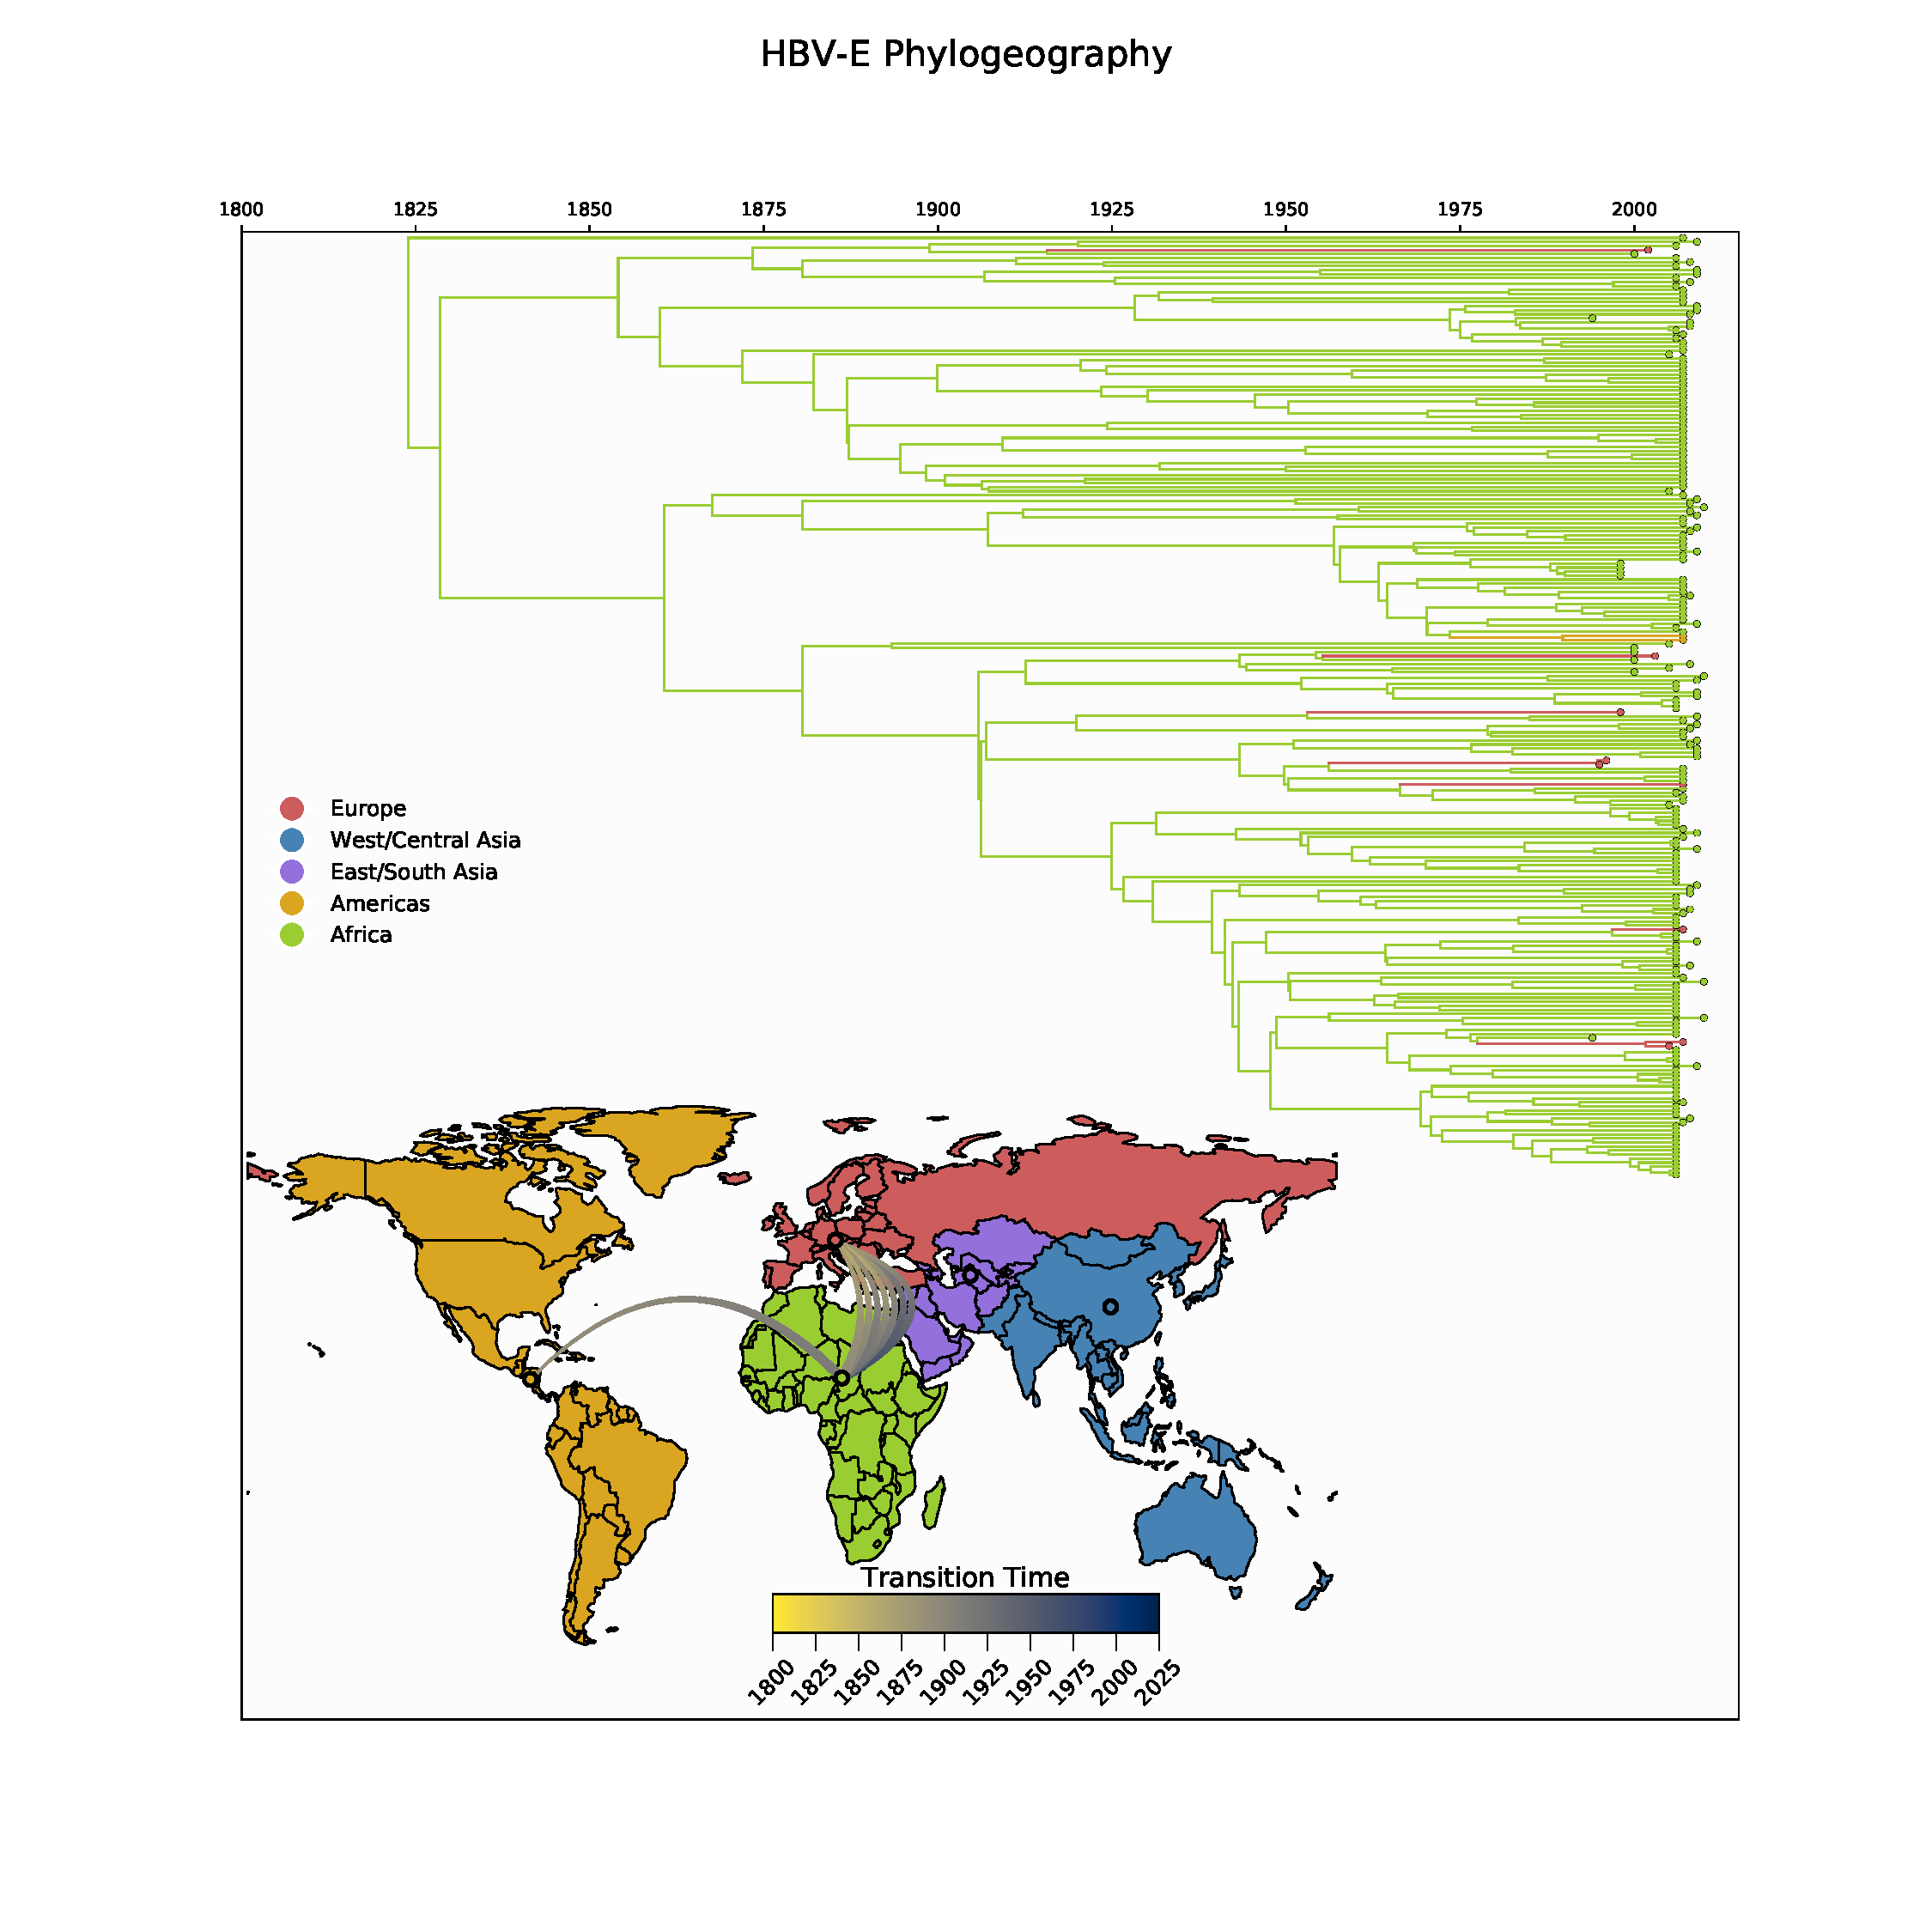
\includegraphics[width=.6\linewidth]{image/results/HBV-E_phylogeography_and_mcc_tree}
  \end{figure}
\end{frame}

%------------------------------------------------
\section{Lassa phylogenetics}
%------------------------------------------------

\begin{frame}
  \frametitle{What is Lassa virus?}
  \begin{columns}[c] % The "c" option specifies centered vertical alignment while the "t" option is used for top vertical alignment

    \column{.45\textwidth} % Left column and width
      \begin{itemize}
        \item Causes $300,000--500,000$ infections annually
        \item Estimated $18\%$ case fatality rate
        \item Segmented RNA virus
        \begin{itemize}
          \item Long segment: ~7.5 kb
          \item Short segment: ~3.5 kb
        \end{itemize}
      \end{itemize}

    \column{.5\textwidth} % Right column and width
      \begin{figure}
        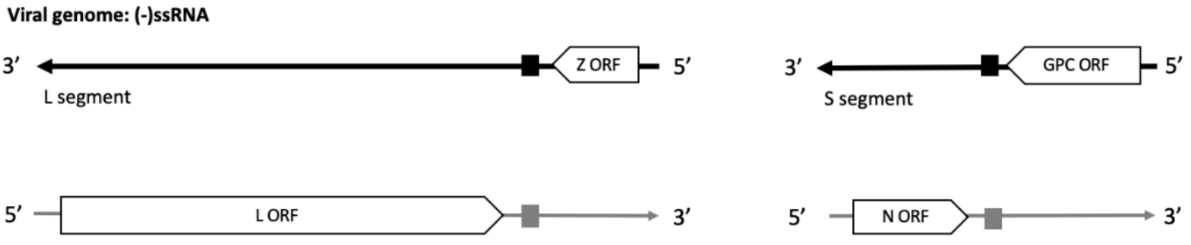
\includegraphics[width=.95\linewidth]{image/intro/lassa_genome_schematic}
        \source{Kafetzopoulou (2019)}
    \end{figure}

  \end{columns}
\end{frame}

%------------------------------------------------
\section{Conclusion}
%------------------------------------------------

\begin{frame}
  \Huge{\centerline{The End}}
\end{frame}

%----------------------------------------------------------------------------------------

\appendix

\begin{frame}
  lipsum
\end{frame}

\begin{frame}
  \frametitle{References}
  \footnotesize{
    \begin{thebibliography}{99} % Beamer does not support BibTeX so references must be inserted manually as below

      \bibitem[Paules, 2017]{paules2017what} Catharine I. Paules, MD; Robert W. Eisinger, PhD; Hilary D. Marston, MD, MPH; and Anthony S. Fauci, MD (2017)
      \newblock What recent hisotory has taught us about responding to emerging infectious disease threats
      \newblock \emph{Annals of Internal Medicinie} 167(11), 805 -- 812.
    \end{thebibliography}

  }

\end{frame}

\end{document}

%--------------------------------------
% EXAMPLE FRAMES
%---------------------------------------

% Highlighted text blocks
% \begin{frame}
%   \frametitle{Blocks of Highlighted Text}
%   \begin{block}{Block 1}
%   Lorem ipsum dolor sit amet, consectetur adipiscing elit. Integer lectus nisl, ultricies in feugiat rutrum, porttitor sit amet augue. Aliquam ut tortor mauris. Sed volutpat ante purus, quis accumsan dolor.
%   \end{block}
%
%   \begin{block}{Block 2}
%   Pellentesque sed tellus purus. Class aptent taciti sociosqu ad litora torquent per conubia nostra, per inceptos himenaeos. Vestibulum quis magna at risus dictum tempor eu vitae velit.
%   \end{block}
%
%   \begin{block}{Block 3}
%   Suspendisse tincidunt sagittis gravida. Curabitur condimentum, enim sed venenatis rutrum, ipsum neque consectetur orci, sed blandit justo nisi ac lacus.
%   \end{block}
% \end{frame}

%------------------------------------------------

% Columns
% \begin{frame}
% \frametitle{Multiple Columns}
% \begin{columns}[c] % The "c" option specifies centered vertical alignment while the "t" option is used for top vertical alignment
%
% \column{.45\textwidth} % Left column and width
% \textbf{Heading}
% \begin{enumerate}
% \item Statement
% \item Explanation
% \item Example
% \end{enumerate}
%
% \column{.5\textwidth} % Right column and width
% Lorem ipsum dolor sit amet, consectetur adipiscing elit. Integer lectus nisl, ultricies in feugiat rutrum, porttitor sit amet augue. Aliquam ut tortor mauris. Sed volutpat ante purus, quis accumsan dolor.
%
% \end{columns}
% \end{frame}

%------------------------------------------------

% Verbatim code
% \begin{frame}[fragile] % Need to use the fragile option when verbatim is used in the slide
% \frametitle{Verbatim}
% \begin{example}[Theorem Slide Code]
% \begin{verbatim}
% \begin{frame}
% \frametitle{Theorem}
% \begin{theorem}[Mass--energy equivalence]
% $E = mc^2$
% \end{theorem}
% \end{frame}\end{verbatim}
% \end{example}
% \end{frame}

%------------------------------------------------

% Math
% \begin{frame}
% \frametitle{Theorem}
% \begin{theorem}[Mass--energy equivalence]
% $E = mc^2$
% \end{theorem}
% \end{frame}

%------------------------------------------------

% Table
% \begin{frame}
% \frametitle{Table}
% \begin{table}
% \begin{tabular}{l l l}
% \toprule
% \textbf{Treatments} & \textbf{Response 1} & \textbf{Response 2}\\
% \midrule
% Treatment 1 & 0.0003262 & 0.562 \\
% Treatment 2 & 0.0015681 & 0.910 \\
% Treatment 3 & 0.0009271 & 0.296 \\
% \bottomrule
% \end{tabular}
% \caption{Table caption}
% \end{table}
% \end{frame}
